\documentclass[12pt]{article}
\usepackage{fontspec}
\usepackage{polyglossia}
\setmonofont{Courier New}
\setmainlanguage{farsi}
\setotherlanguage{english}
\newfontfamily\persianfont[Script=Arabic]{XBZar}
\usepackage{graphicx}
\usepackage{geometry}
\usepackage{hyperref}
\geometry{a4paper, margin=2.5cm}
\usepackage{setspace}
\usepackage{url}
\onehalfspacing
\usepackage{titling}
\usepackage{float}
\usepackage{etoolbox}
\usepackage[backend=biber,style=numeric,sorting=none]{biblatex}
%%%%%%%%%%%%%%%%%%%%%%%%%%%%%%%%%%%%%%%%%%%%%%%%%%%%%%%%%%%%%%%%%%%%%%%%%%%%%
\makeatletter
\newcommand{\persiandigit}[1]{%
	\ifcase#1 ۰\or ۱\or ۲\or ۳\or ۴\or ۵\or ۶\or ۷\or ۸\or ۹\fi
}
\DeclareFieldFormat{labelnumber}{\persiandigit{#1}}
\makeatother
%%%%%%%%%%%%%%%%%%%%%%%%%%%%%%%%%
\newcommand{\persianordinal}[1]{%
	\ifcase#1
	\or اول%
	\or دوم%
	\or سوم%
	\or چهارم%
	\or پنجم%
	\or ششم%
	\or هفتم%
	\or هشتم%
	\or نهم%
	\or دهم%
	\or یازدهم%
	\or دوازدهم%
	\or سیزدهم%
	\or چهاردهم%
	\or پانزدهم%
	\or شانزدهم%
	\or هفدهم%
	\or هجدهم%
	\or نوزدهم%
	\or بیستم%
	\else #1\fi
}

\newcommand{\persianordinalpage}{\persianfont\persianordinal{\value{page}}}


%%%%%%%%%%%%%%%%%%%%%%%%%%%%%%%%%%%%%%%%%%%%%%%%%%%%%%%%%%%%%%%%%%%%%%%%%%%%%
\begin{filecontents}{\jobname.bib}
	@online{a1,
		url = {https://www.wireshark.org/docs/wsug_html_chunked/ChUseStatisticsMenuSection.html}
	}
	@online{a2,
		url = {https://wiki.wireshark.org/TLS}
	}
	@online{a3,
		url = {https://wiki.wireshark.org/RTP_statistics}
	}
	
\end{filecontents}

\addbibresource{\jobname.bib}

\defbibheading{bibliography}[]{%
	\begin{RTL}
		\section*{مراجع}
	\end{RTL}
}

%%%%%%%%%%%%%%%%%%%%%%%%%%%%%%%%%%%%%%%%%%%%%%%%%%%%%%%%%%%%%%%%%%%%%%%%%%%%%

\begin{document}
	
	% ==============================
	% Title Page
	% ==============================
	\begin{titlepage}
		\centering
		\vspace*{1cm}
		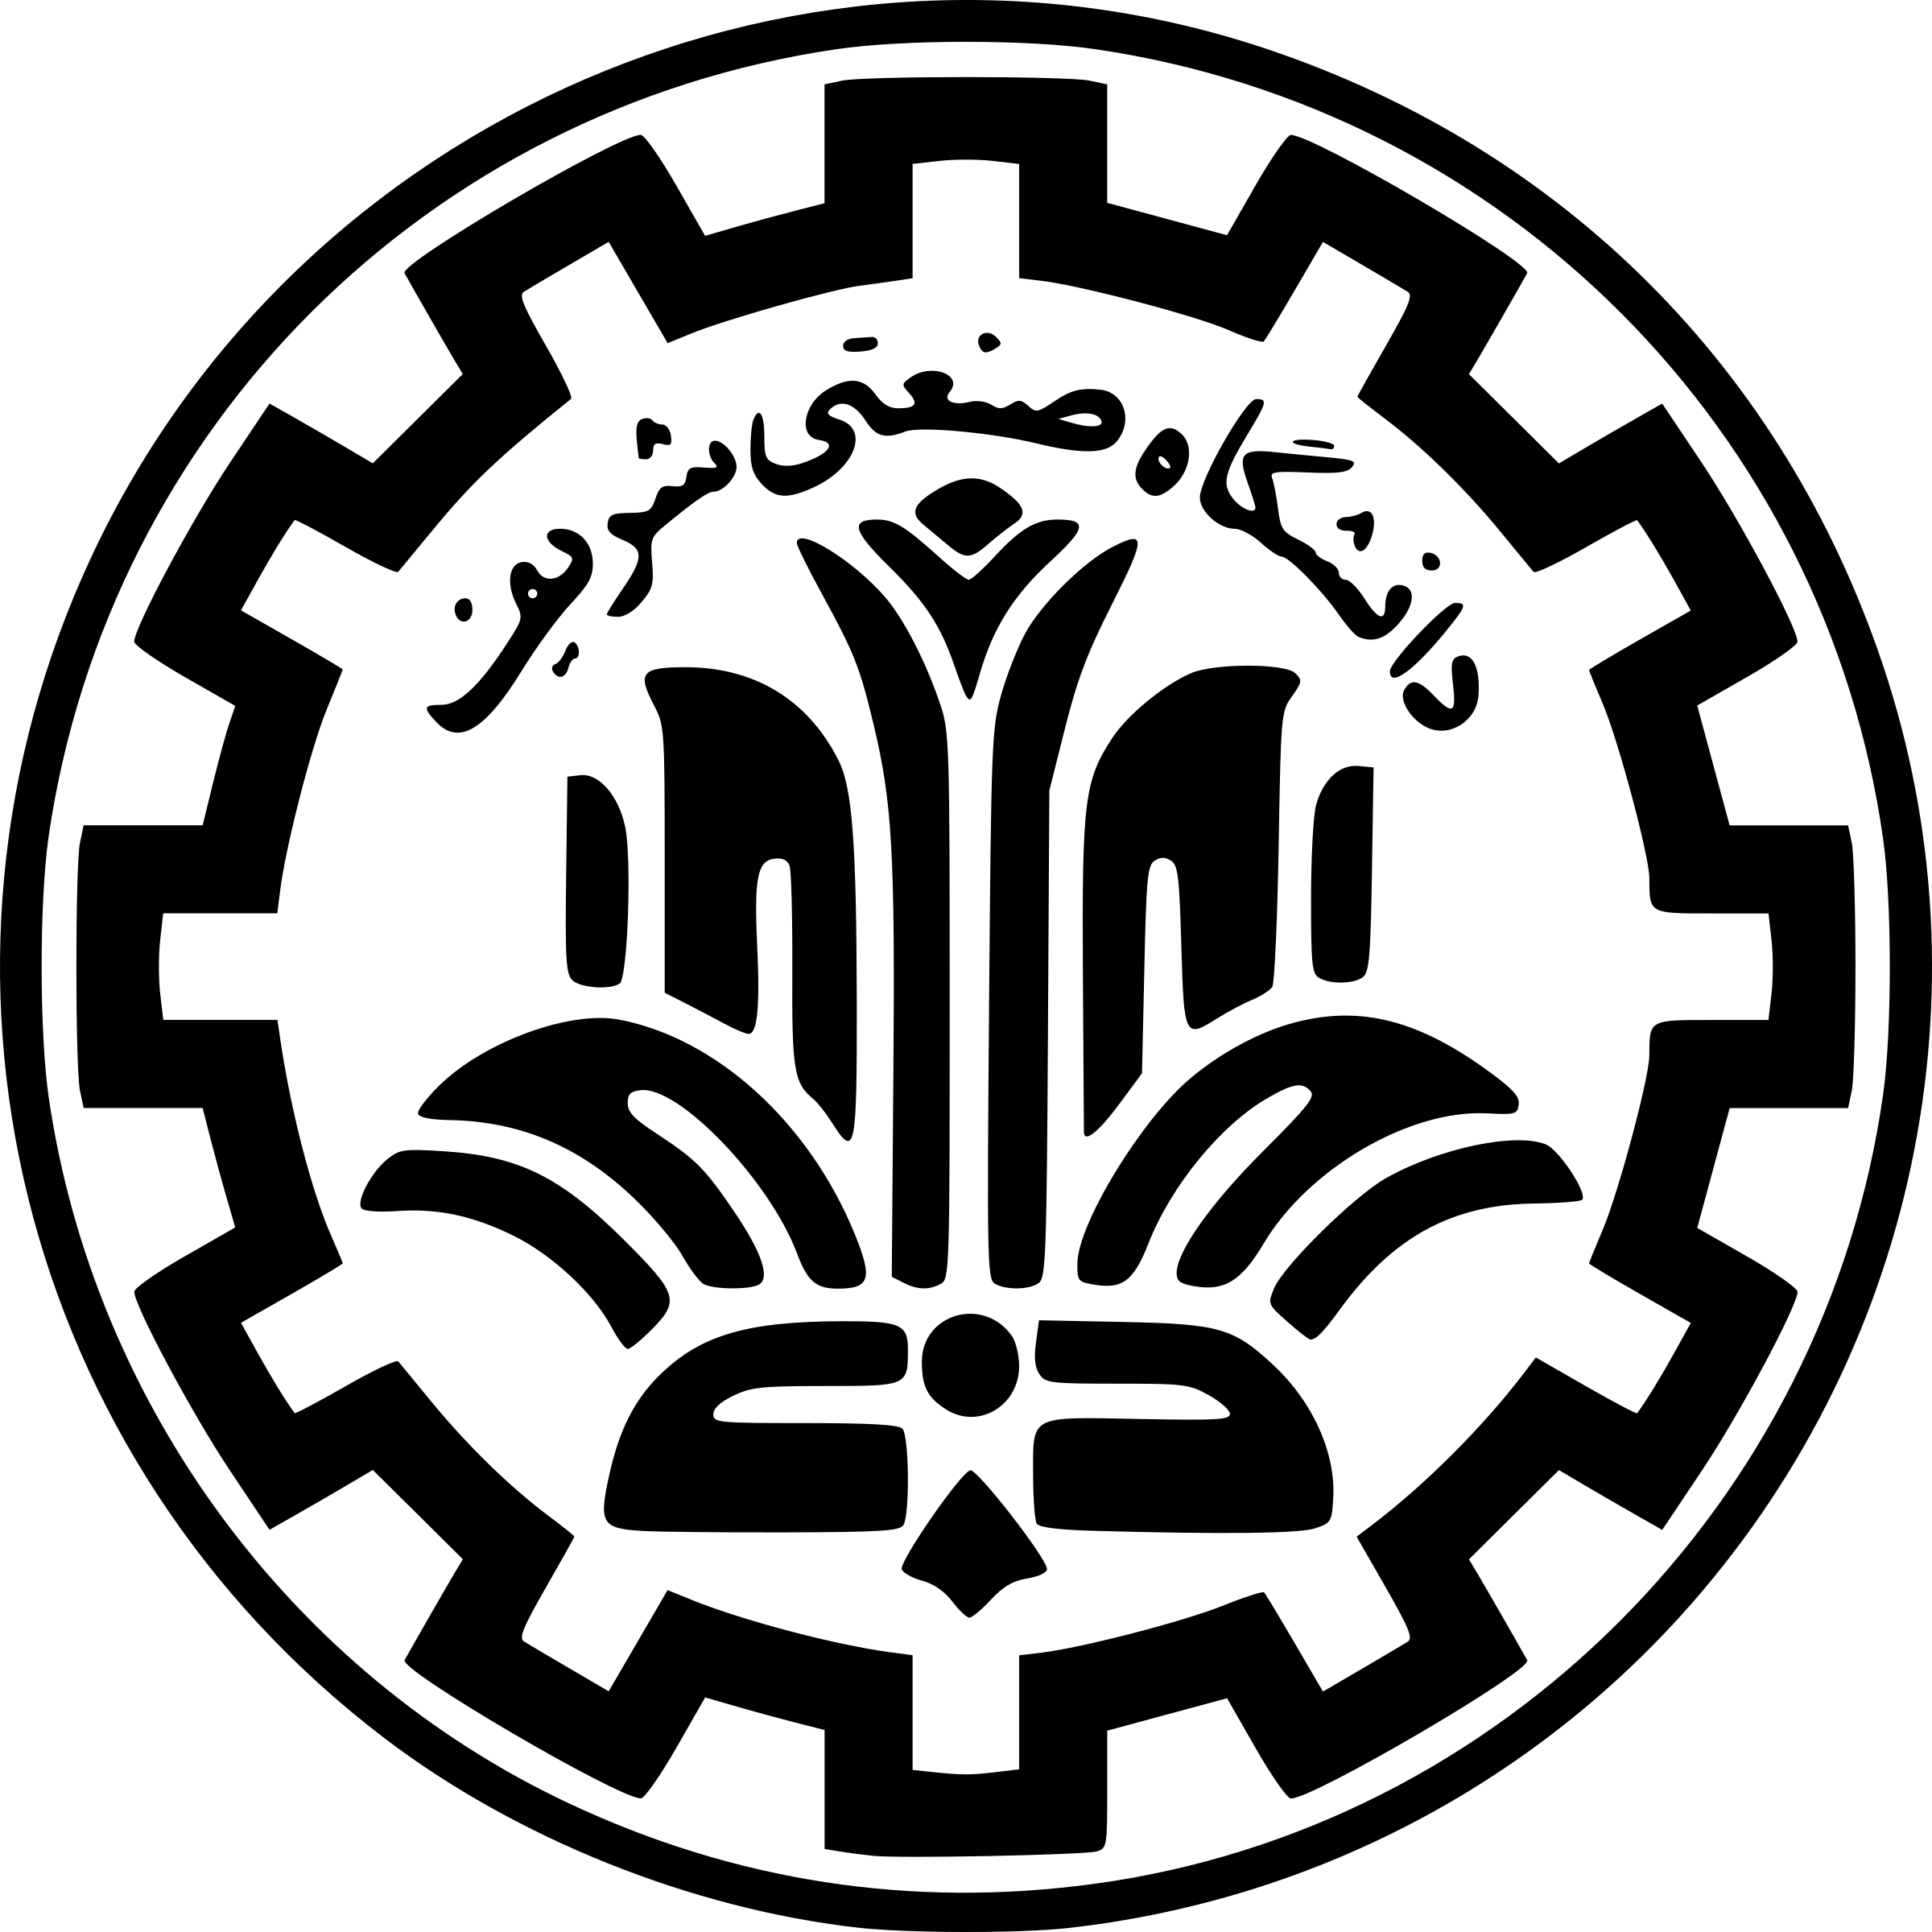
\includegraphics[width=4cm]{sharif.png}\\[1.5cm]
		{\Large\textbf{دانشگاه صنعتی شریف}}\\[0.5cm]
		{\large\textbf{دانشکدهٔ مهندسی کامپیوتر}}\\[1.5cm]
		{\Huge\textbf{گزارش کار آزمایشگاه}}\\[0.5cm]
		{\LARGE\textbf{آزمایشگاه شبکه‌های کامپیوتری}}\\[2cm]
		
		\textbf{گزارش آزمایش شماره ۳}\\
		(‫آشنایی ‬‫پیشرفته‬ ‫با‬ ‫نرم‌افزار \textenglish{ٌWireshark}، نحوهٔ ‬‫تنظیم‬ \textenglish{‫‪Server‬‬ ‫‪DNS}‬‬)
		
		\vfill
		\begin{tabular}{rl}
			\textbf{شمارهٔ گروه:} & ۴ \\
			\textbf{گروه:} &
			ارشیا یوسف‌نیا (۴۰۱۱۱۰۴۱۵) \\
			& محمد‌فرحان بهرامی (۴۰۱۱۰۵۷۲۹) \\
			& امیرمهدی دارایی (۹۹۱۰۵۴۳۱) \\
			\textbf{استاد درس:} & دکتر صفایی \\
			\textbf{تاریخ:} & تابستان ۱۴۰۴ \\
		\end{tabular}
	\end{titlepage}
	
	% ==============================
	% Persian Ordinal Page Numbering
	% ==============================
	\clearpage
	\setcounter{page}{1}
	\renewcommand{\thepage}{\persianordinalpage}
	
	\tableofcontents
	\clearpage
	\listoffigures
	\clearpage
	\listoftables
	
	% ==============================
	% Switch to Persian Digits (۱, ۲, ۳, ...)
	% ==============================
	\clearpage
	\setcounter{page}{1}
	\pagenumbering{arabic}
	\renewcommand{\thepage}{\persianfont\arabic{page}}
	
	
	% ==============================
	% Main Content
	% ==============================
	\section{wireshark}
	\subsection{بازیابی کپچا}
	فایل مورد نظر را در نرم‌افزار باز می‌کنیم، در ادامه طبق شکل \ref{cap:1} فایل رمز جلسه را در قسمت پروتکل TLS وارد می‌کنیم تا بتوانیم بسته‌های رمز شده را رمزگشایی کنیم. در نهایت با فیلتر موجود در شکل \ref{cap:2} تنها این پیام‌ها را نشان می‌دهیم و فایل‌ها را از این پیام‌ها خروجی می‌گیریم. در شکل \ref{cap:2} این فایل‌ها و حاصل کار آمده. شکل \ref{cap:3} هم کد کپچا را جداگانه نشان می‌دهد. پس کد امنیتی p94kuq بوده.
	 
	\begin{figure}[h]
		\centering
		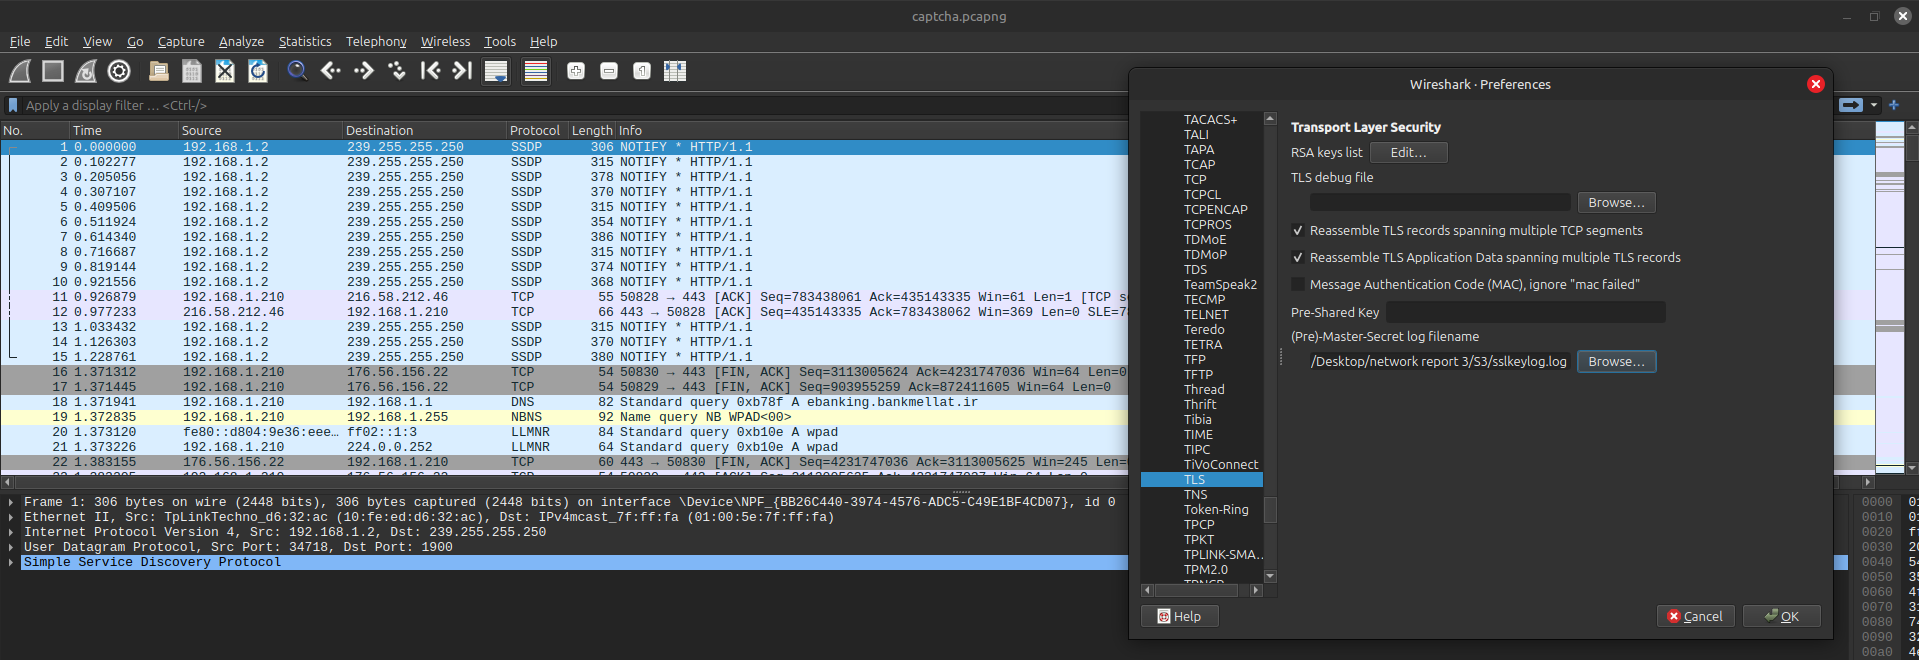
\includegraphics[width=\textwidth]{resources/1.png}
		\caption{باز کردن فایل و وارد کردن فایل نشست در بخش TLS}
		\label{cap:1}
	\end{figure}
	\begin{figure}[h]
		\centering
		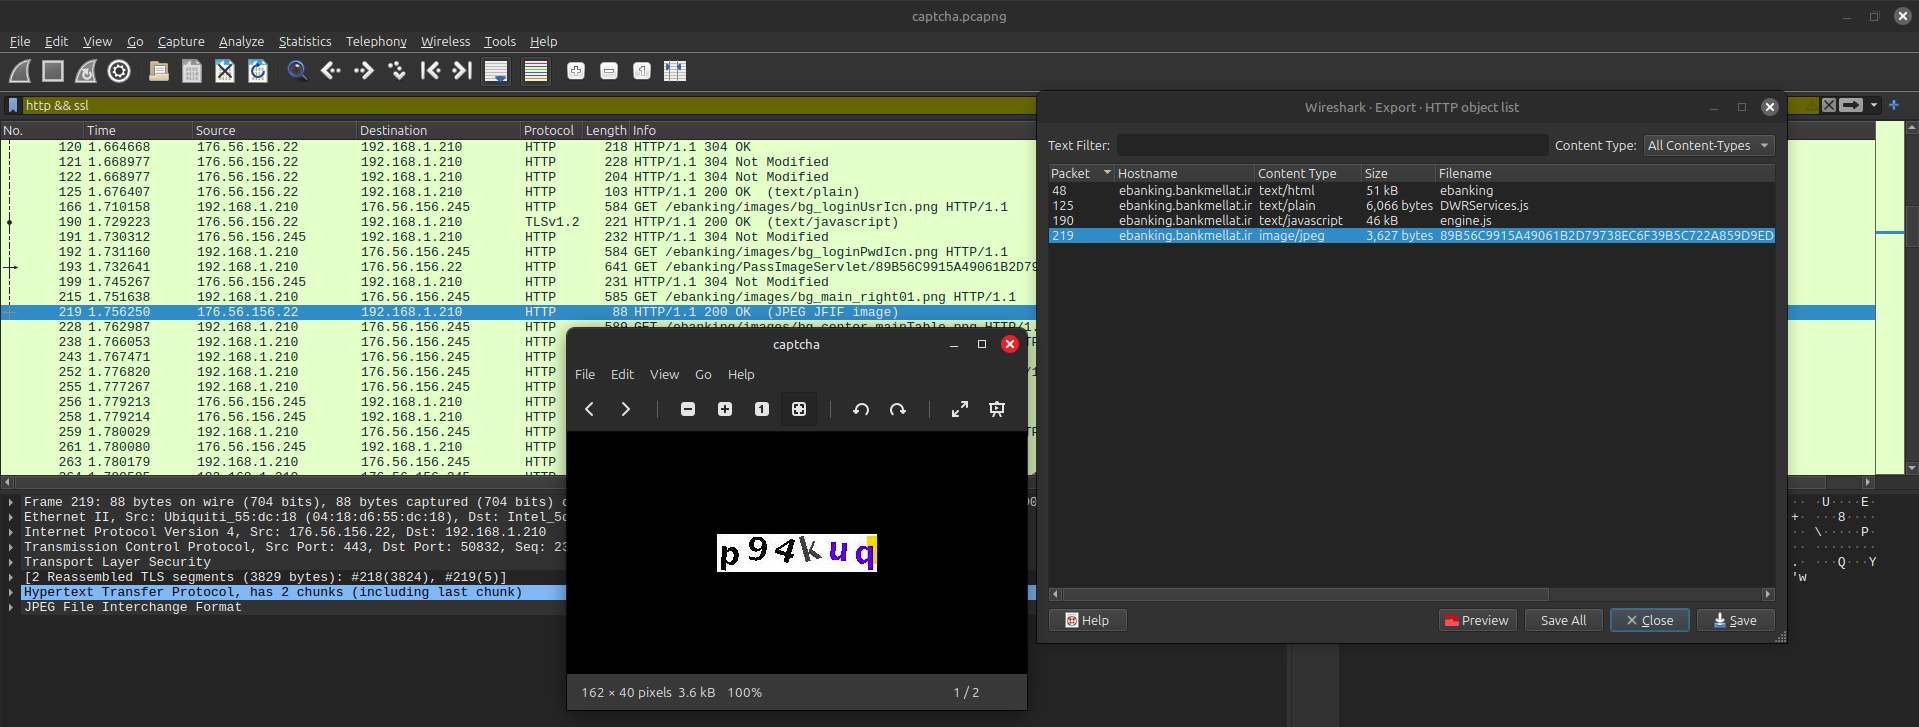
\includegraphics[width=\textwidth]{resources/2.png}
		\caption{اعمال فیلتر در نمایش و خروجی گرفتن از فایل‌های رمزگشایی شده}
		\label{cap:2}
	\end{figure}
	\begin{figure}[h]
		\centering
		
\includegraphics[width=0.2\textwidth]{resources/captcha.png}
		\caption{کپچای استخراج شده از فایل بسته‌ها}
		\label{cap:3}
	\end{figure}
	
	
	\subsection{سوال‌ها}
	
	\subsubsection{}
	Wireshark
	 دسترسی به اطلاعات آماری بسته‌ها را از طریق منوی "Statistics" فراهم می‌کند. این ابزارها برای تحلیل ترافیک شبکه، حتی در شرایطی که کلید جلسه برای بسته‌های رمزنگاری‌شده در دسترس نیست، بسیار مفید هستند. بر اساس مستندات \textenglish{Wireshark}، ابزارهای آماری شامل مواردی که در جدول \ref{wire:1} آمده هستند.
	 \begin{table}[h]
	 	\centering
	 	\begin{tabular}{|l|p{4cm}|p{4cm}|}
	 		\hline
	 		ابزار آماری & توضیحات & کاربردها \\
	 		\hline
	 		\textenglish{Protocol Hierarchy} & نمایش سلسله مراتبی از پروتکل‌ها و درصد استفاده هر کدام & تحلیل توزیع پروتکل‌ها و شناسایی ترافیک غالب \\
	 		\hline
	 		\textenglish{Conversations} & لیست گفتگوها (ترافیک بین دو نقطه پایانی) & ردیابی الگوهای ارتباطی و شناسایی ناهنجاری‌ها \\
	 		\hline
	 		\textenglish{Endpoints} & لیست نقاط پایانی (ترافیک به و از یک آدرس) & شناسایی دستگاه‌های فعال و ارزیابی حجم ترافیک \\
	 		\hline
	 		\textenglish{Packet Lengths} & تحلیل توزیع اندازه بسته‌ها & شناسایی بسته‌های غیرمعمول و بهینه‌سازی شبکه \\
	 		\hline
	 		\textenglish{I/O Graphs} & نمودارهای سفارشی برای نمایش ترافیک در طول زمان (مثلاً تعداد بسته‌ها) & مشاهده روندها و عیب‌یابی مشکلات عملکرد \\
	 		\hline
	 		\textenglish{Service Response Time} & اندازه‌گیری زمان بین درخواست و پاسخ برای خدمات & ارزیابی تأخیر برنامه‌ها و اطمینان از کارایی \\
	 		\hline
	 	\end{tabular}
	 	\caption{ابزارهای آماری در Wireshark}
	 	\label{wire:1}
	 \end{table}
	 این ابزارها به کاربران اجازه می‌دهند بدون نیاز به رمزگشایی محتوای بسته‌ها، الگوهای ترافیک را تحلیل کنند. برای نمونه، اگر کلید جلسه برای بسته‌های رمزنگاری‌شده (مانند \textenglish{TLS}) در دسترس نباشد، همچنان می‌توان حجم داده‌ها، فرکانس ارتباطات و پروتکل‌های استفاده‌شده را بررسی کرد. این قابلیت برای عیب‌یابی شبکه، برنامه‌ریزی ظرفیت و نظارت امنیتی بسیار مفید است.
	 
	 در مورد رمزگشایی \textenglish{TLS}، Wireshark برای رمزگشایی نیاز به کلیدهای خاصی مانند فایل لاگ کلید (\textenglish{Key Log File})، کلید خصوصی RSA یا کلید پیش‌به‌اشتراکی (PSK) دارد. بدون این کلیدها، رمزگشایی ممکن نیست، اما ابزارهای آماری همچنان قابل استفاده هستند و اطلاعات ارزشمندی دارند.
	 
	 مراجع این بخش \cite{a1, a2} است.
	\subsubsection{}
	پروتکل \textenglish{RTP (Real-time Transport Protocol)} یک پروتکل استاندارد برای انتقال داده‌های بی‌درنگ مانند صدا و ویدیو از طریق شبکه‌های IP است. این پروتکل معمولاً بر روی UDP اجرا می‌شود و برای کاربردهایی مانند VoIP، پخش زنده و کنفرانس ویدیویی استفاده می‌شود. RTP همراه با پروتکل کنترل RTCP برای نظارت بر تحویل داده‌ها کار می‌کند.
	Wireshark
	 ابزارهای پیشرفته‌ای برای تحلیل ترافیک RTP ارائه می‌دهد که در جدول \ref{wire:2} به آنها اشاره شده است.
	 \begin{table}[h]
	 	\centering
	 	\begin{tabular}{|p{3cm}|p{5cm}|p{5cm}|}
	 		\hline
	 		ویژگی & توضیحات & جزئیات/یادداشت‌ها \\
	 		\hline
	 		تحلیل جریان RTP & تحلیل آماری جریان‌های RTP از طریق منوی
	 		 \textenglish{Telephony > RTP > Show All Streams}
	 		 ، شامل تأخیر، جیتر، پهنای باند، از دست رفتن بسته‌ها و خطاهای توالی. & شامل نمودار برای نمایش جیتر و تفاوت‌های بسته‌ها در طول زمان. \\
	 		\hline
	 		محاسبه جیتر & محاسبه بر اساس RFC3550، فرمول:
	 		
	 		 $J(i) = J(i-1) + (|D(i-1,i)| - J(i-1))/16$
	 		 
	 		 ، نیاز به فرکانس نمونه‌برداری (مثلاً 8000 هرتز برای \textenglish{G.711}). & مثال: G.711 PCMA با فرکانس 8000 هرتز، واحد $0.000125$ ثانیه. \\
	 		\hline
	 		محاسبه پهنای باند & نمایش پهنای باند در سطح IP، شامل هدرهای IP (20 بایت) و UDP (8 بایت) در ثانیه اخیر. & رجوع به تابع rtp\_packet\_analyse در tap-rtp-common.c. \\
	 		\hline
	 		ذخیره جریان‌های صوتی RTP & ذخیره صدا در فایل Au از منوی تحلیل جریان RTP، پشتیبانی از کدک‌هایی با فرکانس 8000 هرتز (از نسخه $3.2.0$، قبلاً فقط \textenglish{G.711}). & گزینه‌ها: همگام‌سازی فایل، همگام‌سازی جریان، بدون همگام‌سازی. \\
	 		\hline
	 		پشتیبانی از کدک‌های دیگر & ذخیره در فرمت rtpdump برای کدک‌های دیگر، پخش با rtplay از rtptools، G.729 به دلیل هزینه مجوز پشتیبانی نمی‌شود. & مثال: پخش با JMstudio، آدرس IP محلی (نه $127.0.0.1$). \\
	 		\hline
	 	\end{tabular}
	 	\caption{ویژگی‌های تحلیل RTP در Wireshark}
	 	\label{wire:2}
	 \end{table}
	 
	 این ابزارها به کاربران اجازه می‌دهند مشکلات رایج مانند جیتر بالا، از دست رفتن بسته‌ها یا تأخیر زیاد را شناسایی کنند. برای نمونه، تحلیل جیتر می‌تواند کیفیت تماس‌های صوتی را ارزیابی کند، و ذخیره جریان‌های صوتی برای بازتولید و تحلیل بیشتر مفید است. مستندات نشان می‌دهد که یک جیتر کمتر از ۳۰ میلی‌ثانیه برای ترافیک صوتی قابل قبول است، و تأخیر یک‌طرفه کمتر از ۱۵۰ میلی‌ثانیه برای VoIP مناسب است.
	 
	 منبع \cite{a3}
	\section{راه‌اندازی \textenglish{DNS}}
	این قسمت بر روی \textenglish{Linux Mint 22.1 'Xia'} انجام شده است.\\
	ابتدا bind9 را نصب میکنیم، همچنین در همین ابتدا دستورات کلیدی دیگر برای راه‌اندازی سرویس و بازنمایی آن آمده است.
	
	\begin{english}
		sudo apt install bind9 bind9utils bind9-doc dnsutils
	\end{english}
	
	\begin{english}
		sudo systemctl start named
	\end{english}
	
	\begin{english}
		sudo systemctl restart named
	\end{english}
	
	\subsection{سناریو آزمایش}
	یک منطقه به نام netlaba4.edu می‌سازیم. سرور نام یا nameserver آن را در ns.netlaba4.edu میگذاریم که ip برابر با 192.168.88.1 است. دو زیرمنطقه هم با نام‌های group1 و group2 به ترتیب با آدرس ip برابر 192.168.88.11 و 192.168.88.22 است. هر دو زیردامنه نام مستعار هم دارند که جزییات آن در ادامه می‌آید. برای جستجوی معکوس هم رکورد‌ها اضافه شده است.
	
	در شکل \ref{dns:1} محتوای
	 /etc/bind/named.conf.local
	  که مربوط به منطقه و رکورد‌های معکوس است آمده.
	\begin{figure}[H]
		\centering
		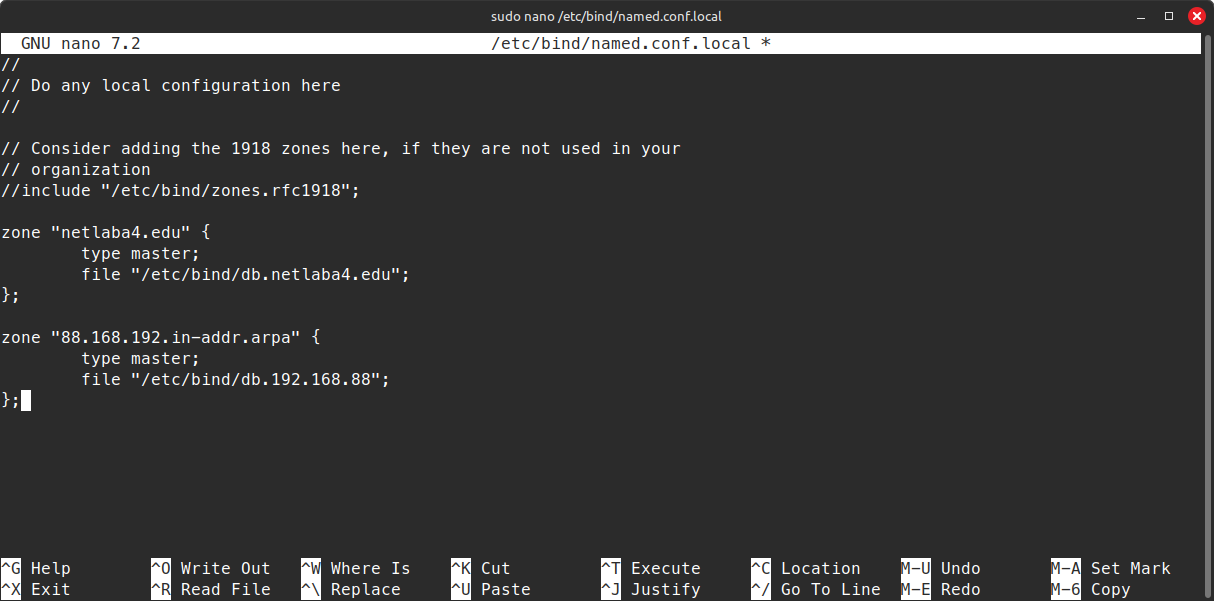
\includegraphics[width=\textwidth]{resources/3.png}
		\caption{تنظمیات اصلی منطقه و رکورد‌های معکوس، نوع آنها و محل فایل رکورد‌ها.}
		\label{dns:1}
	\end{figure}
	در ادامه رکوردهای SOA و NS و A و CNAME را برای دو منطقه و دو زیردامنهٔ خود در
	 /etc/bind/db.netlaba4.edu 
	وارد می‌کنیم، در شکل \ref{dns:2}‌ جزییات آمده است.
	\begin{figure}[H]
		\centering
		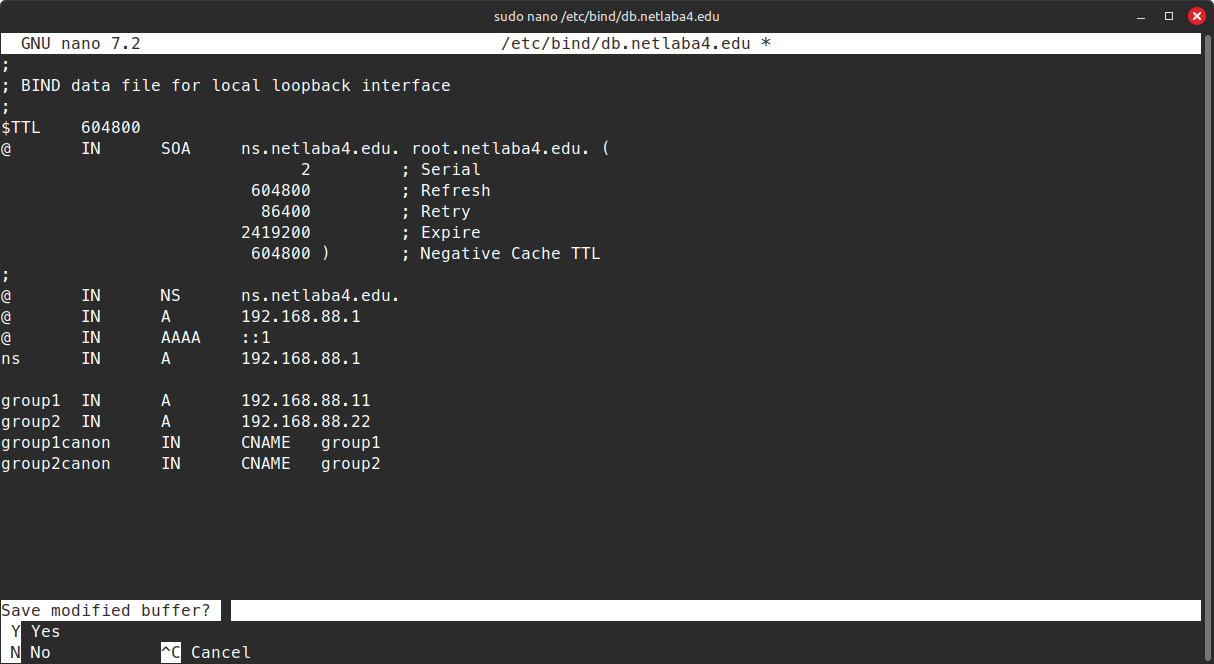
\includegraphics[width=\textwidth]{resources/4.png}
		\caption{تنظمیات اصلی منطقه و رکورد‌های معکوس، نوع آنها و محل فایل رکورد‌ها.}
		\label{dns:2}
	\end{figure}
	در شکل \ref{dns:3} در
	 /etc/bind/db.192.168.88
	  به رکورد‌های مربوط به پرسش‌های معکوس می‌پردازیم.
	\begin{figure}[H]
		\centering
		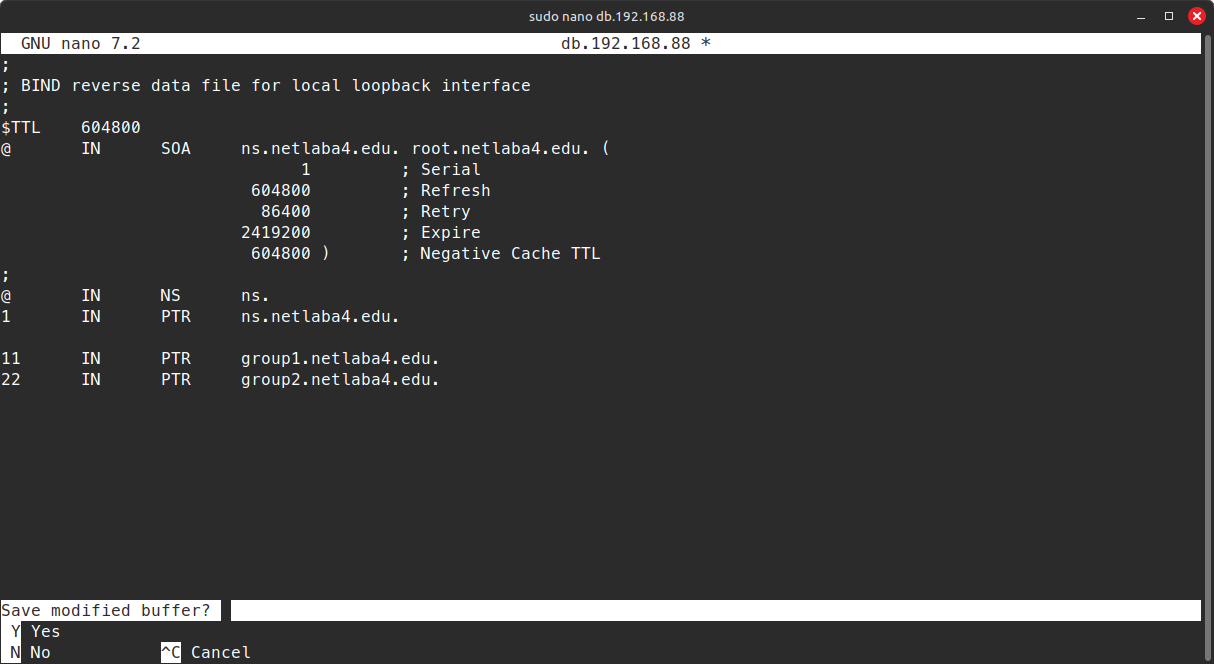
\includegraphics[width=\textwidth]{resources/5.png}
		\caption{وارد کردن رکورد‌های اصلی، سرور نام، آدرس آیپی، و نام‌های مستعار}
		\label{dns:3}
	\end{figure}
	حالا باید کاری کنیم این سرویس در پرسش‌ها مورد توجه قرار گیرد. شکل \ref{dns:4} در
	 /etc/resolv.conf
	  این کار را انجام می‌دهد.
	\begin{figure}[H]
		\centering
		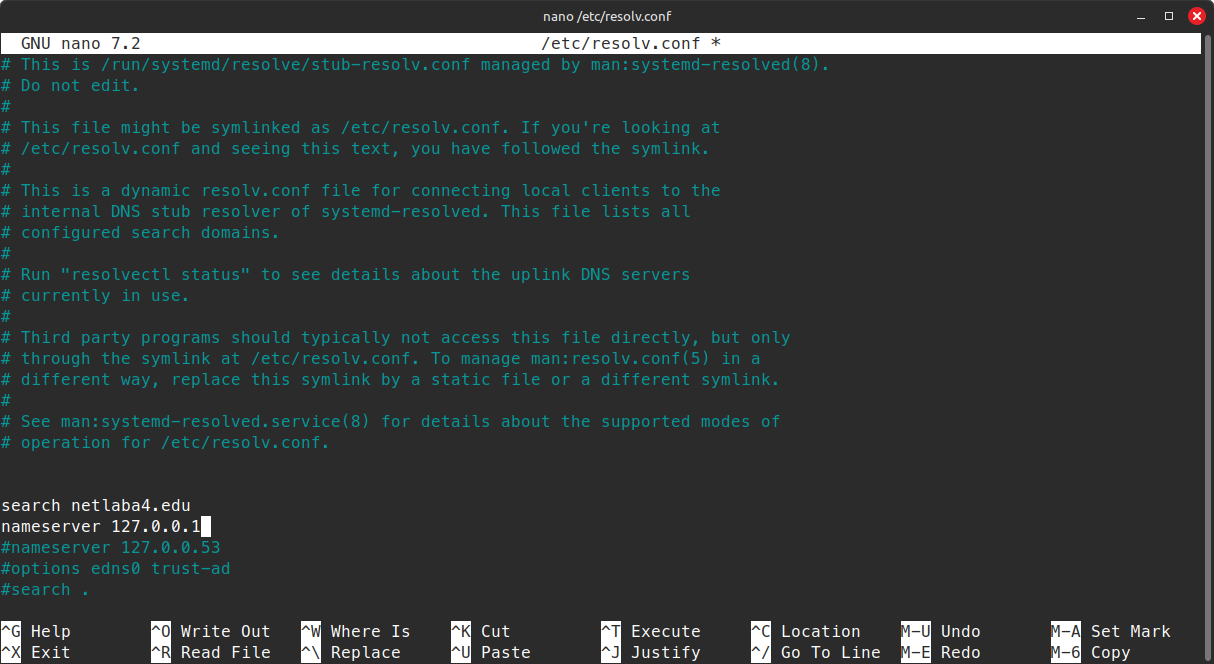
\includegraphics[width=\textwidth]{resources/6.png}
		\caption{وارد کردن رکورد‌ها برای پرسش‌های معکوس}
		\label{dns:4}
	\end{figure}
	
	در نهایت با دستور‌های آمده در ابتدای این بخش سرویس‌ها را restart می‌کنیم که در شکل
	 \ref{dns:5}
	 آمده است. در ادامه باید نتایج را آزمایش ‌کنیم و همزمان نرم‌افزار wireshark را هم روی واسط loopback به حالت capture قرار می‌دهیم. 
	\begin{figure}[H]
		\centering
		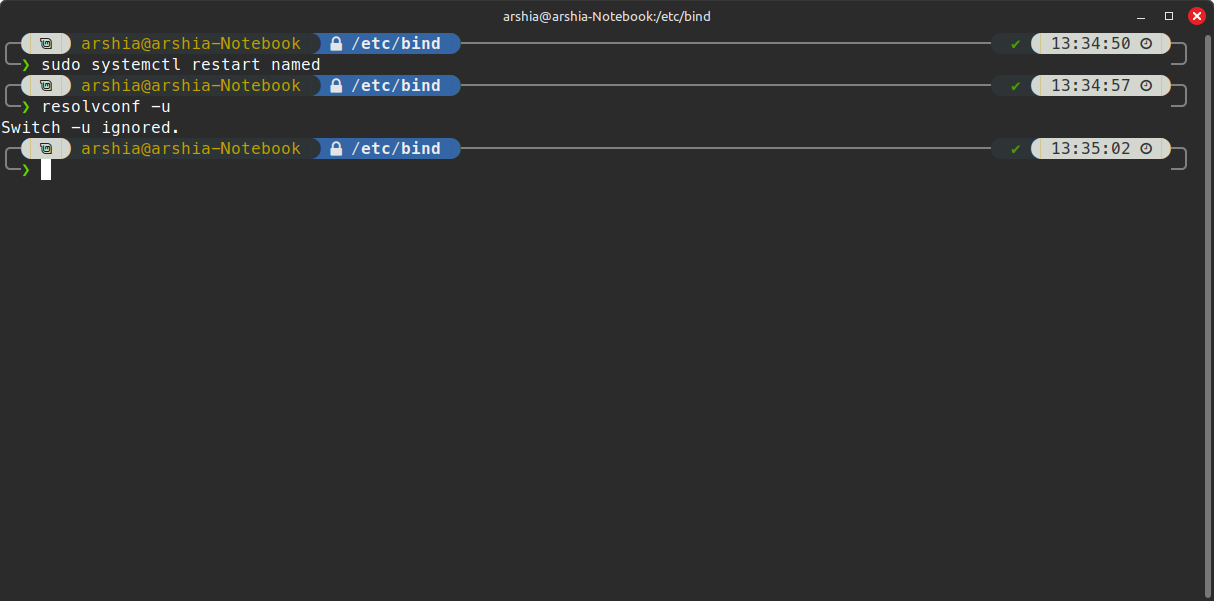
\includegraphics[width=\textwidth]{resources/7.png}
		\caption{آماده کردن سرویس bind برای در نظر گرفته شدن در سوال‌ها}
		\label{dns:5}
	\end{figure}
	پرسش‌های مستقیم با nslookup در شکل \ref{dns:6} و پرسش‌های معکوس در شکل \ref{dns:7} به همراه پاسخ‌ها آمده است.
	\begin{figure}[H]
		\centering
		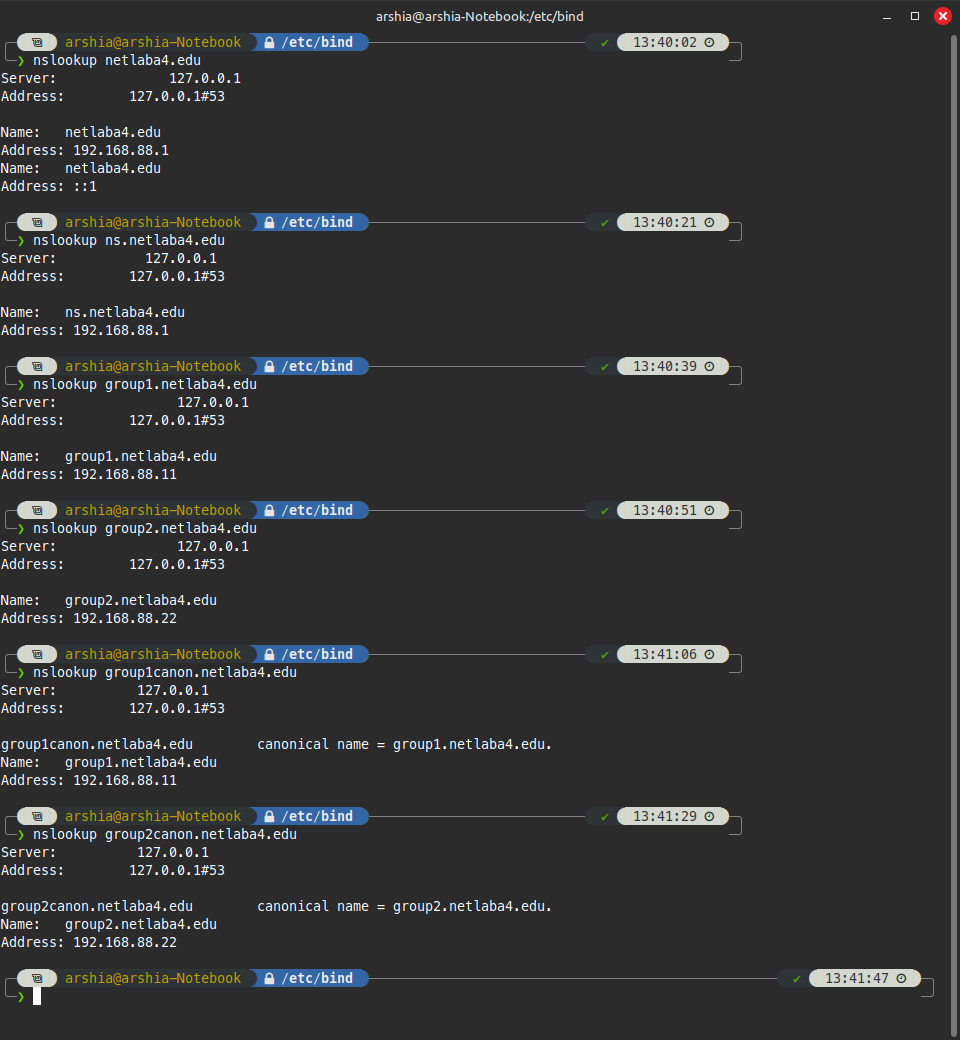
\includegraphics[width=\textwidth]{resources/8.png}
		\caption{پرسش و پاسخ‌های مستقیم با nslookup}
		\label{dns:6}
	\end{figure}
	\begin{figure}[H]
		\centering
		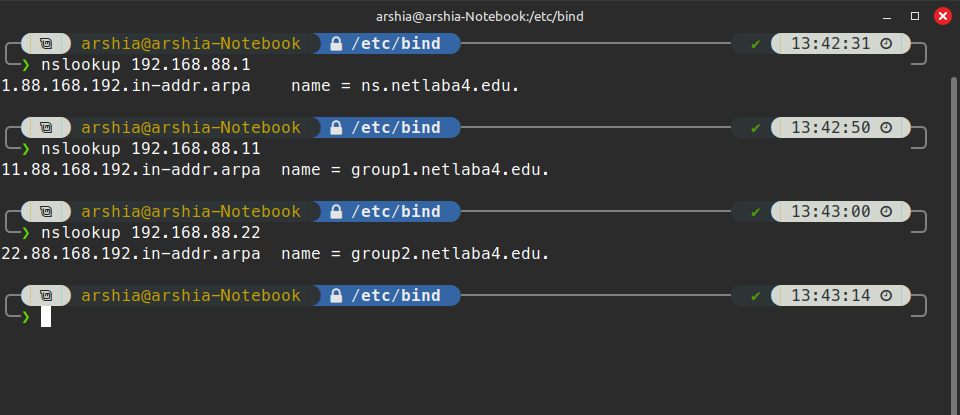
\includegraphics[width=\textwidth]{resources/9.png}
		\caption{پرسش و پاسخ‌های وارونه با nslookup}
		\label{dns:7}
	\end{figure}
	\subsection{پرسش‌ها}
	\subsubsection{}
	همانطور که در شکل \ref{dns:8} آمده، متناظر با هر پرسش با nslookup یک بسته با پروتکل DNS ارسال شده و به ازای جواب آن هم یک بسته آمده است که رفتار مورد انتظار DNS است. 
	\begin{figure}[H]
		\centering
		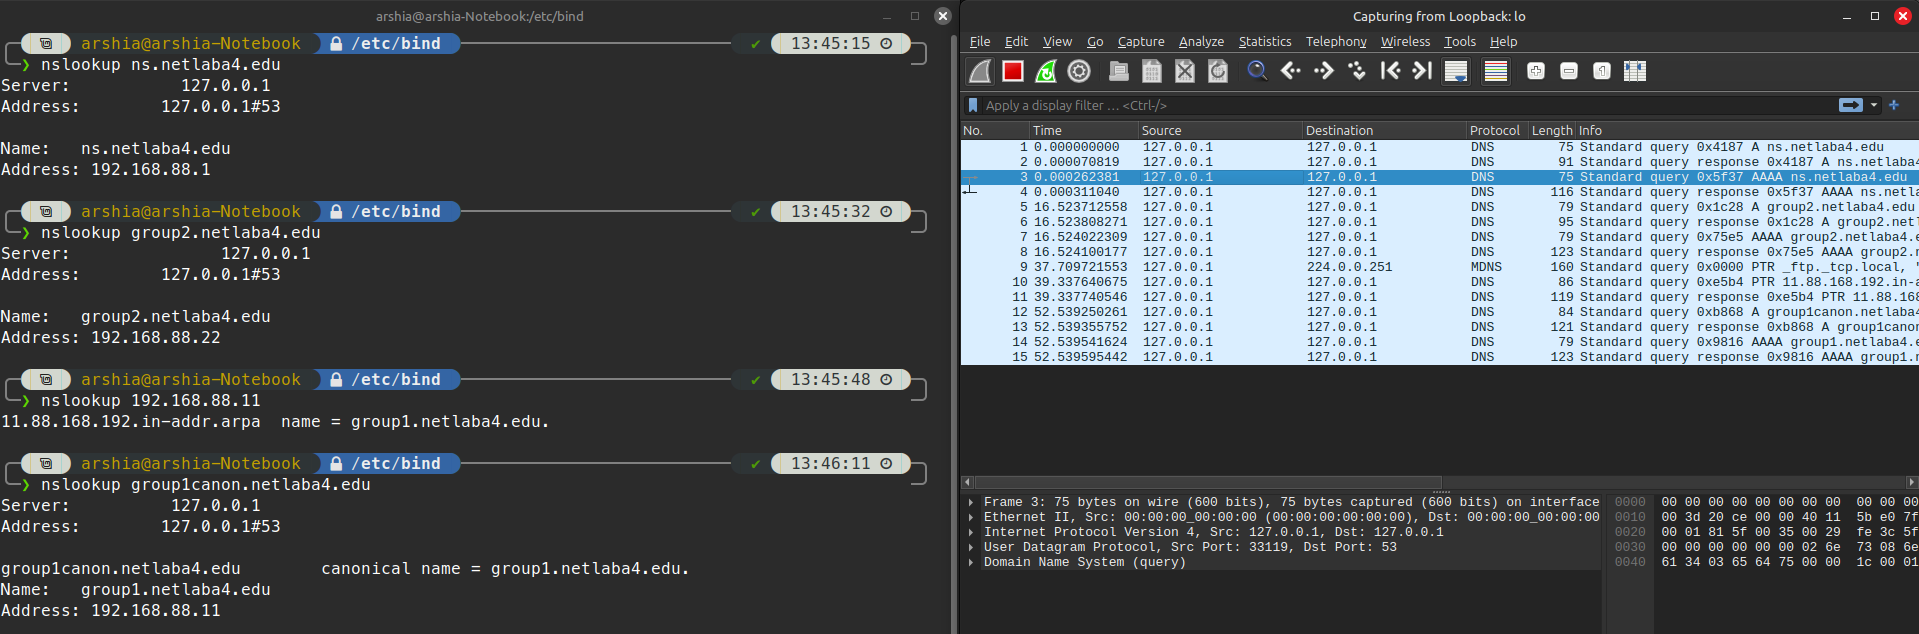
\includegraphics[width=\textwidth]{resources/10.png}
		\caption{پرسش و پاسخ‌های  nslookup و بسته‌های ردگیری شدهٔ نرم‌افزار wireshark از این ارتباط}
		\label{dns:8}
	\end{figure}
	\subsubsection{}
	در شکل‌های \ref{dns:9}، \ref{dns:10}، و \ref{dns:11} ۳ نوع از پرسش‌های مختف را آورده‌ایم، پرسش‌های مستقیم به دنبال آدرس آیپی بوده‌اند که بیشتر نسخهٔ ۴ بوده، پس در پرسش و پاسخ متناظر A آمده است، به همین ترتیب برای آیپی نسخهٔ ۶ نیز AAAA آمده است. در نهایت برای پرسش‌های وارونه که به دنبال آیپی از روی نام هستند هم نوع PTR یا \textenglish{domain name PoinTer} آمده است.
	\begin{figure}[H]
		\centering
		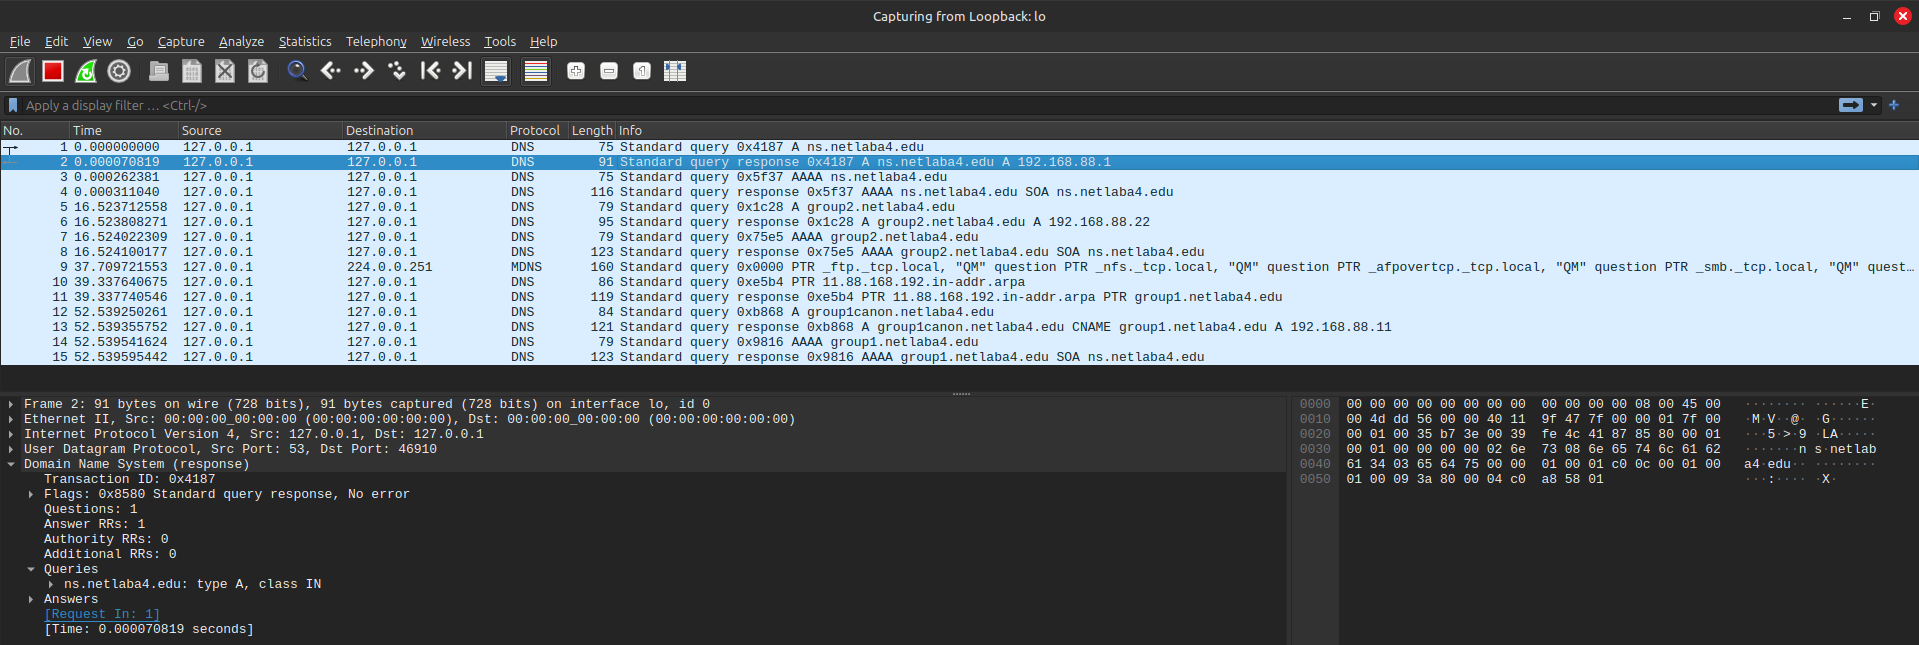
\includegraphics[width=\textwidth]{resources/11.png}
		\caption{یک پرسمان با نوع رکورد A}
		\label{dns:9}
	\end{figure}
	\begin{figure}[H]
		\centering
		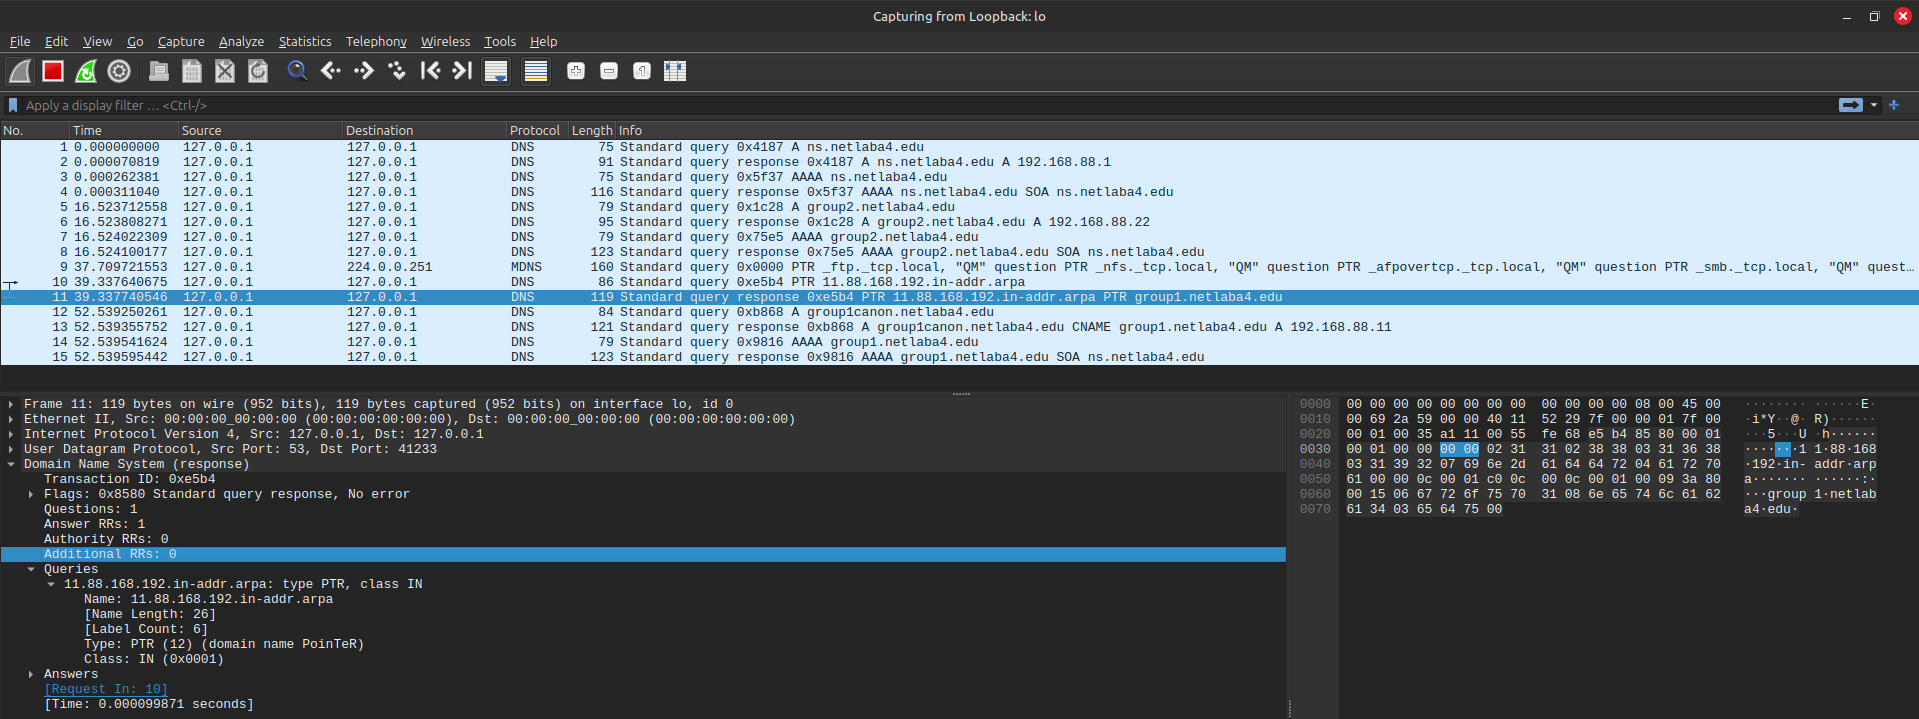
\includegraphics[width=\textwidth]{resources/12.png}
		\caption{یک پرسمان با نوع رکورد PTR}
		\label{dns:10}
	\end{figure}
	\begin{figure}[H]
		\centering
		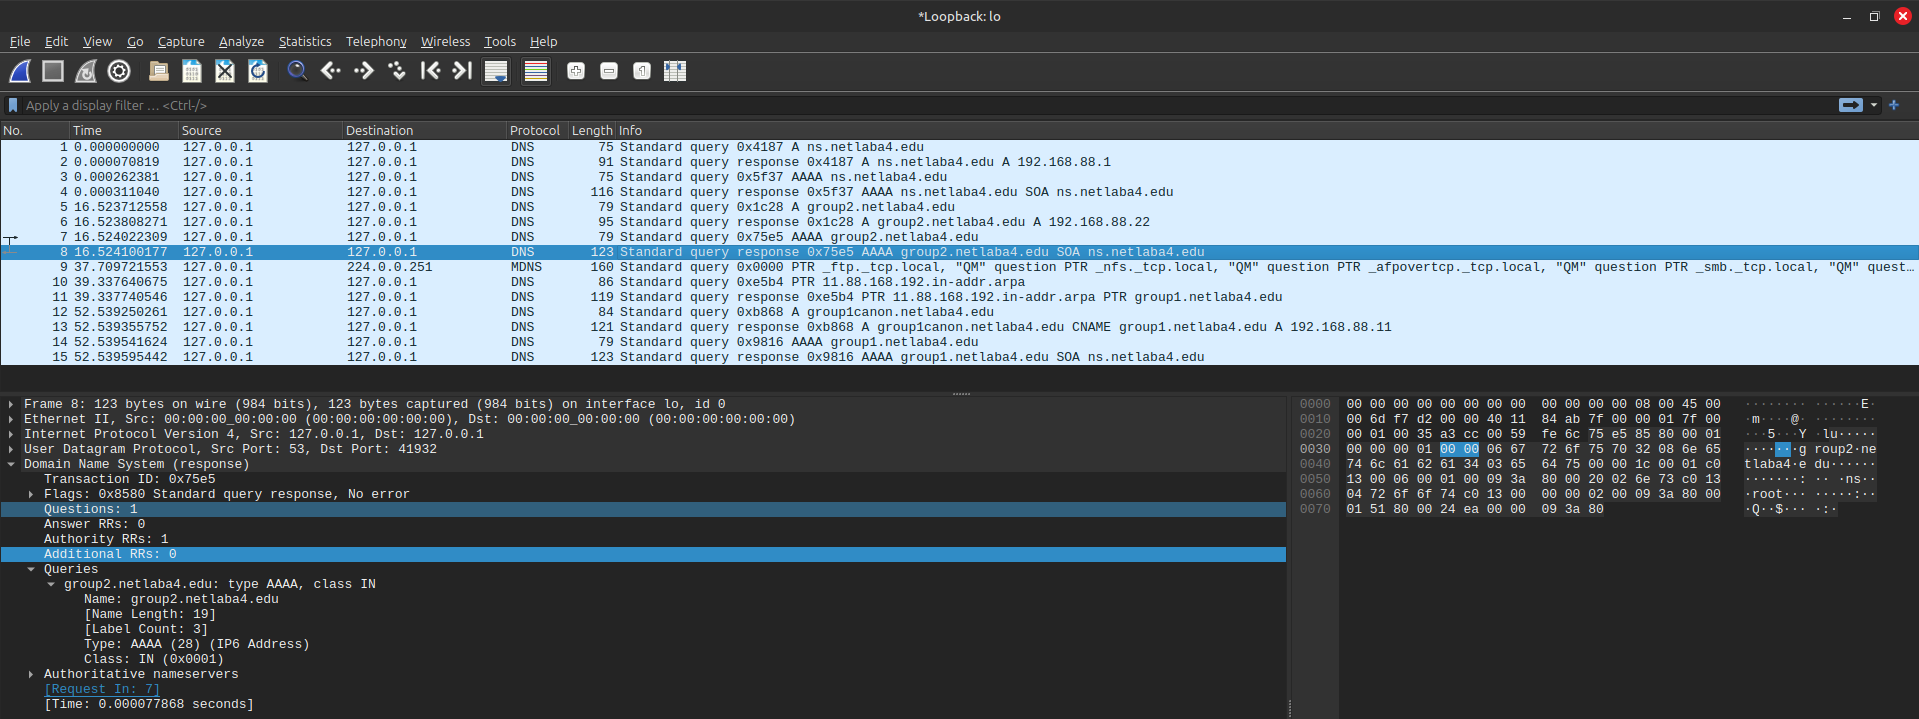
\includegraphics[width=\textwidth]{resources/13.png}
		\caption{یک پرسمان با نوع رکورد AAAA}
		\label{dns:11}
	\end{figure}
	
	% ==============================
	% References
	% ==============================
	\newpage
	\begin{LTR}
		\printbibliography[title={مراجع}]
	\end{LTR}
	
\end{document}
